\documentclass[10pt, conference, letterpaper]{IEEEtran}

\usepackage{graphicx}
\usepackage{caption}

% *** SUBFIGURE PACKAGES ***
\usepackage{subfig}

\usepackage{blindtext}
\usepackage{adjustbox}
\usepackage{multirow}
\usepackage{color}
\usepackage{booktabs}
\usepackage{tabularx}
\usepackage{colortbl}
\usepackage{bbding}
\usepackage{tikz}
\usepackage{listings}
\usepackage{etoolbox}
\usepackage{subfig}

\usepackage{url}
\usepackage{setspace}
%\usepackage{enumitem}
\usepackage[british,english]{babel}


%\usepackage[caption=false,font=footnotesize]{subfig}


\newcommand{\circled}[2][]{\tikz[baseline=(char.base)]
    {\node[shape = circle, draw, inner sep = 1pt]
    (char) {\phantom{\ifblank{#1}{#2}{#1}}};%
    \node at (char.center) {\makebox[0pt][c]{#2}};}}
\robustify{\circled}


\newcommand\FIXME[1]{\textcolor{red}{FIX:}\textcolor{red}{#1}}

\makeatletter
\def\@IEEEsectpunct{.\ \,}
\def\paragraph{\@startsection{paragraph}{4}{\z@}{1.5ex plus 1.5ex minus 0.5ex}%
{0ex}{\normalfont\normalsize\sffamily\bfseries}}


\patchcmd{\@maketitle}
  {\addvspace{0.2\baselineskip}\egroup}
  {\addvspace{-1\baselineskip}\egroup}
  {}
  {}

\makeatother


\begin{document}

\title{Deep learning
\vspace{-4 mm}}



\author{\IEEEauthorblockN{Qq\IEEEauthorrefmark{2}}
\IEEEauthorblockA{
\IEEEauthorrefmark{2}Northwest University, China, \IEEEauthorrefmark{3}Lancaster University, UK \\
\IEEEauthorrefmark{2} jr@stumail.nwu.edu.cn, \{gl, hwang\}@nwu.edu.cn, \IEEEauthorrefmark{3}z.wang@lancaster.ac.uk
\vspace{-3 mm}
}
}

\maketitle
\begin{abstract}

\end{abstract}

% Note that keywords are not normally used for peerreview papers.
\begin{IEEEkeywords}
workload characterisation
\end{IEEEkeywords}

\section{Introduction}
In recent years, deep learning has emerged as a powerful tool for solving problems that were considered to be difficult in the past. It has
demonstrated impressive results on tasks like object recognition~\cite{donahue14,he2016deep}, facial
recognition~\cite{parkhi2015deep,sun2014deep}, speech processing~\cite{pmlrv48amodei16}, and machine translation~\cite{bahdanau2014neural}.
While many of these tasks are also important on mobiles and the Internet of Things (IoT), existing solutions are often
computation-intensive and require a large amount of resources for the model to operate. Performing deep inference\footnote{Inference in
this paper refers to apply a pre-trained model on an input to obtain the corresponding output. This is different from statistical
inference.} on embedded devices can lead to long runtimes and the consumption of abundant amounts of resources, including CPU, memory, and
power, even for simple tasks~\cite{CanzianiPC16}. Without a solution,
 the hoped-for advances on embedded sensing will not arrive.


Numerous approaches have been proposed to accelerate deep inference on embedded devices. These include designing specialize hardware to
reduce the computation or memory latency~\cite{}, compressing a pre-trained model to reduce its storage and memory footprint as well as
computational requirements~\cite{}, and offloading some, or all, computation to a cloud
server~\cite{Kang2017neurosurgeon,teerapittayanon2017distributed}. Compared to specialized hardware, software-based model compression
techniques have the advantage of being readily deployable on commercial-off-the-self hardware and compared to computation offloading, model
compression enables on-device inference which in turn allows faster response time and has less privacy concerns. These advantages make
model compressions attractive on existing hardware platform where computation offloading is not feasible.


However, model compression is not a free lunch as it comes at the cost of loss in prediction accuracy~\cite{}. This means that one must
carefully choose the model compression technique and its parameters to effectively trade precision for computation and resource
requirements. Furthermore, as we will show in this paper, the reduction in the model size does not necessarily translate into faster
inference time. Because a model compression technique is not always beneficial, it is important to understand when and how to apply a
 technique.

In this paper, we aim to understand model compression techniques for embedded inference. Having this knowledge allows not only better
deployment of computation-intensive models on mobile and IoT devices, but also designing more efficient architectures for models and
hardware acceleration.

In this work, we conducted extensive experiments to evaluate two mainstream model compression techniques, pruning~\cite{Li2016Pruning} and data
quantization~\cite{Gong2014Compressing}. We apply model compression techniques to the image classification domain, an area where deep learning has made
impressive breakthroughs and a rich set of pre-trained models are available. We evaluate our approach on the NVIDIA Jetson TX2 embedded
deep learning platform and consider a wide range of influential DNN models. Our experiments are performed using the 50K images from the
ImageNet ILSVRC 2012 validation dataset.

We show that while there may be significant gain for choosing the right compression technique and parameters, mistakes can seriously hurt
the performance. We show how different model compression techniques and parameters affect the inference time, model storage requirement and
the prediction accuracy. As a result, our work provides insights on when and how to apply deep learning model compression techniques on
embedded devices.

The main contributions of this paper are two folds:

\begin{itemize}
\item We present an extensive study to characterize and understand how two popular model compression techniques perform on a
    representative embedded deep learning platform;
\item Our work offers insights on when and how to apply compression techniques for embedded deep inference.
\end{itemize}

\section{Motivation}


%The JavaScript engine's performance that involves the compiler,
%garbage collector, etc., and the final display work on GPU are separate issues beyond the scope of this work.

\begin{table}[!t]
\caption{The best-performing available governor}
\vspace{-3mm}
\scriptsize
\begin{center}
        \begin{tabular}{llll}
        \toprule
        &\textbf{Load time}&\textbf{Energy}&\textbf{EDP}\\
        \midrule
            Regular 3G                     &\Performance&\Powersave&\Powersave\\
            \rowcolor{Gray}Regular 4G                     &\Performance&\Conservative&\Interactive\\
            WiFi            &\Interactive&\Ondemand&\Interactive\\
        \bottomrule
        \end{tabular}
\end{center}
\label{tab:best-governor}
\vspace{-5mm}
\end{table}


\begin{figure}[!t]
	\centering
	\subfloat[][Load time]{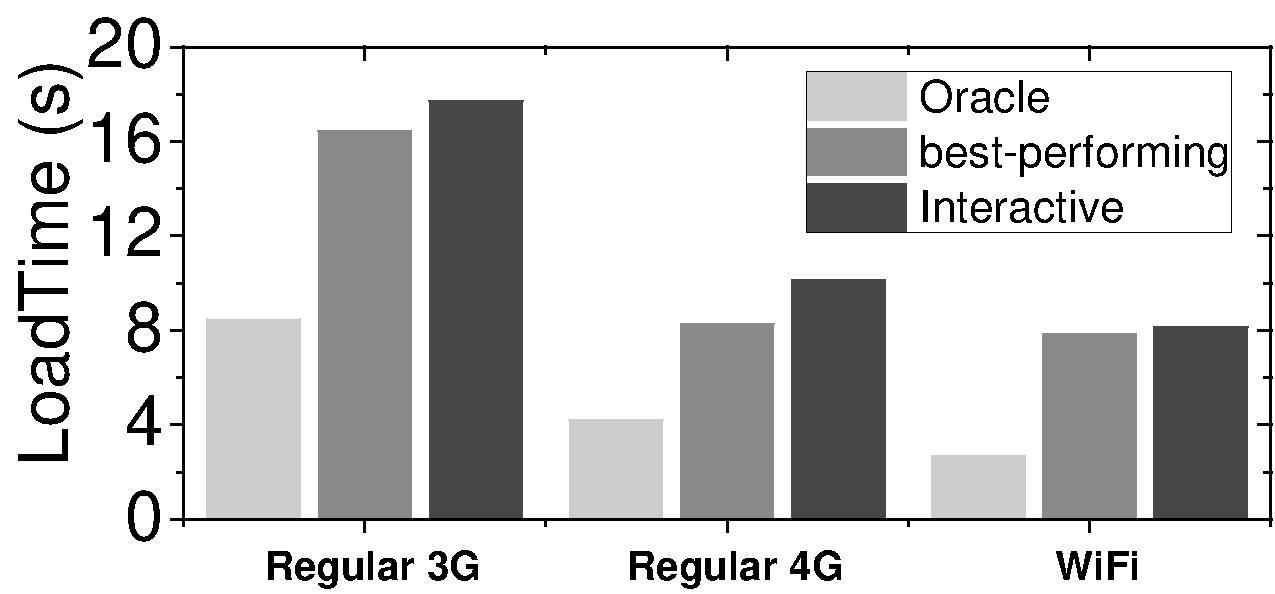
\includegraphics[width=0.22\textwidth]{figure/laod4pagesloadtime.pdf}}
    \hfill
    \subfloat[][Energy consumption]{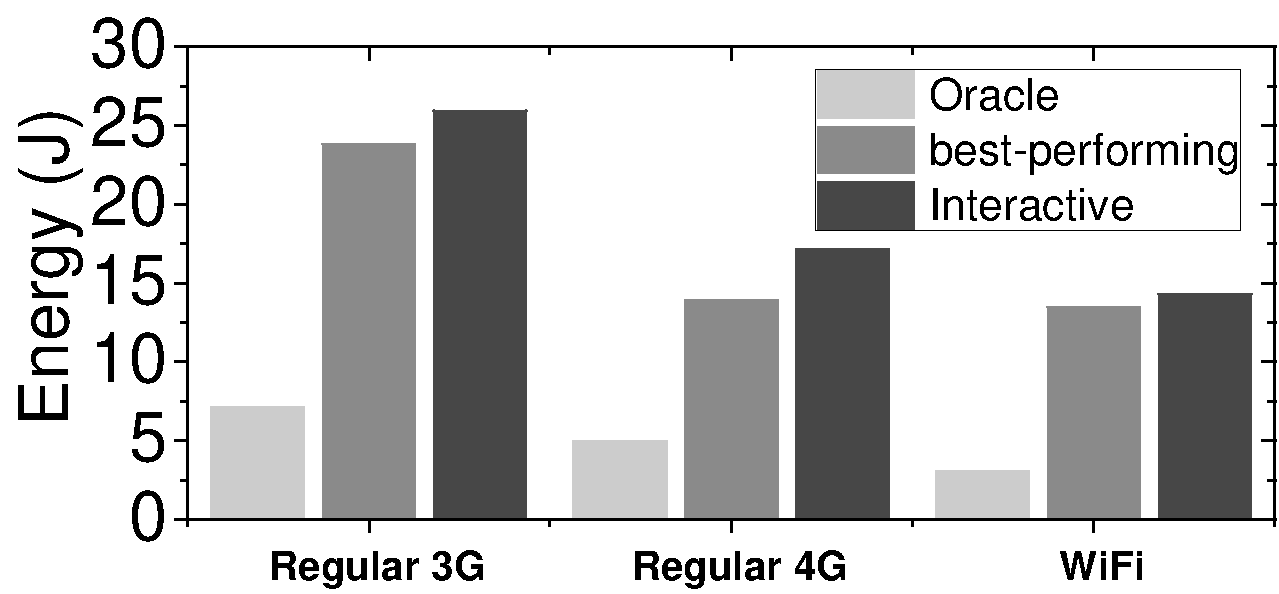
\includegraphics[width=0.22\textwidth]{figure/load4pagesEnergy.pdf}}
    \vspace{-2mm}
    \caption{The achieved total load time (a), energy consumption (b)  when a user was browsing four news pages from \BBCW.
    We show the results for \Oracle, the \bfp existing CPU frequency governor, and \Interactive in three typical networking environments. There is significant room for improvement. }
    \vspace{-5mm}
    \label{fig:motivation}
\end{figure}



Consider a scenario for browsing four \texttt{BBC} news pages, starting from the home page of \BBCW. Our evaluation platform has  a
Cortex-A15 (big) and a Cortex-A7 (little) processors.

\vspace{-1mm}
\cparagraph{Networking Environments.} We consider three typical networking
environments: Regular 3G, Regular 4G and WiFi (see Section~\ref{sec:networks} for more details). To ensure reproducible results, web requests and responses are deterministically replayed by the client and a web server respectively. The
web server simulates the download speed and latency of a given network setting, and we record and deterministically replay the
user interaction trace for each testing scenario.


\vspace{-1mm}
\cparagraph{Scheduling Strategies.} We schedule the Chromium rendering engine (i.e., \texttt{CrRendererMain}) to run on either the big or the little
core under different clock frequencies to find the best processor configuration per test case. We refer this best-found configuration as
the \Oracle because it is the best performance we can get via CPU frequency scaling and task mapping. We use the \Interactive CPU
frequency governor as the baseline, which is the default frequency governor on many mobile devices \cite{Seo2015Big}. We also compare with the best-performing governor found from mainstream CPU governors,
including
the \Interactive and other four strategies: \Performance, \Conservative, \Ondemand and \Powersave.


 %We evaluate the performance of each strategy in three typical networking environments, Regular 3G, Regular 4G,
%and WiFi, where a typical smartphone user would  experience. Table~\ref{tab:network} shows the configuration of each networking environment setting.
%Later in this paper, we evaluate our approach on a wider range of networking environments (see Section~\ref{}).

\cparagraph{Motivation Results.} Table~\ref{tab:best-governor} lists the best-performing governor chosen from the five existing CPU
frequency governors, and Figure~\ref{fig:motivation} summarizes the performance of each strategy for each optimization metric. While
\Interactive  gives the best \EDP compared to other existing governors in a Regular 4G and a WiFi environments, it fails to deliver the
best-available performance for load time and energy consumption. Furthermore, there is significant room for improvement for the best-performing
existing governor when compared to the \Oracle.  On average, the \Oracle outperforms the best-performing governor by 154.6\%,
70.6\% respectively for load time and energy consumption across networking environments.
More importantly, the oracle processor configuration varies across web pages, networking
environments and evaluation metrics -- no single configuration consistently delivers the best-available performance.

\cparagraph{Lessons Learned.} This example shows that the current mainstream CPU frequency governors are ill-suited for mobile web browsing
and the best processor configuration depends on the network and the optimization goal. There is a need for a better scheduler that can
adapt to the webpage workload, the networking environment and the optimization goal. In the remainder of this article, we describe such an
approach based on machine learning.

\section{Workloads}

\input{Overview}
\section{System Evaluation\label{sec:evaluation}}

\section{Related Work}
\DNNs have shown astounding successes in various tasks that previously seemed difficult~\cite{}. Despite the fact that many embedded
devices require precise sensing capabilities, adoption of \DNN models on such systems has notably slow progress. This mainly due to
\DNN-based inference being typically a computation intensive task, which inherently runs slowly on embedded devices due to limited
resources.

\FIXME{Talk about different compression techniques.}

There is an extensive body of work on how to accelerate \DNN training using xx, xx, and xx. Our work aims to understand how to accelerate
deep learning inference by choosing the right model compression technique.


As an alternative to on-device inferencing, off-loading computation to the cloud can accelerate \DNN model inference
\cite{teerapittayanon2017distributed}. Neurosurgeon \cite{Kang2017neurosurgeon} identifies when it is beneficial (\eg in terms of energy
consumption and end-to-end latency) to offload a \DNN layer to be computed on the cloud. The Pervasive \CNN~\cite{7920809} generates
multiple computation kernels for each layer of a \CNN, which are then dynamically selected according to the inputs and user constraints. A
similar approach presented in \cite{RodriguezWZMH17} trains a model twice, once on shared data and again on personal data, in an attempt to
prevent personal data being sent outside the personal domain. Computation off-loading is not always applicable due to privacy, latency or
connectivity issues. The work presented by Ossia \etal partially addresses the issue of privacy-preserving when offloading \DNN inference
to the cloud ~\cite{ossia2017hybrid}. Our work is complementary to prior work on computation off-loading by offering insights to choose the
optimal compression technique to best optimize local inference.

\section{Conclusions}
This paper has presented an automatic approach to optimize the mobile web



\newcommand{\BIBdecl}{\setlength{\itemsep}{0.3 em}}
\bibliographystyle{IEEEtran}
\bibliography{IEEEabrv,refs}

\end{document}
